\xiti
\begin{xiaotis}

\xiaoti{在一个斜坡上,沿着与坡脚的水平线成 $45^\circ$ 角的直道上坡。如果行走 40 米后升高了 14.14 米,求坡面的倾斜度。}

\xiaoti{有两个二面角,它们的面对应平行。求证:它们的棱互相平行。 这两个二面角的大小有怎样的关系?}

\xiaoti{在一个二面角的一个面内有一点,它到棱的距离等于到另一个面的距离的 2 倍。求二面角的度数。}

\xiaoti{要铣一个 V 形铁。 V 形面成直二面角,上口宽 40 mm。求切削深度。}

\begin{figure}[htbp]
    \centering
    \begin{minipage}[b]{7cm}
        \centering
        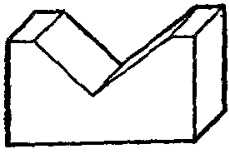
\includegraphics[width=4cm]{../pic/ltjh-ch1-xiti6-04.png}
        \caption*{(第 4 题)}
    \end{minipage}
    \qquad
    \begin{minipage}[b]{7cm}
        \centering
        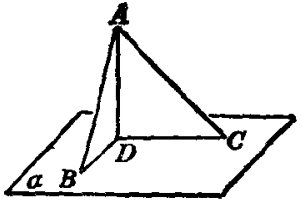
\includegraphics[width=5cm]{../pic/ltjh-ch1-xiti6-08.png}
        \caption*{(第 8 题)}
    \end{minipage}
\end{figure}

\xiaoti{在 $45^\circ$ 二面角的一个面内有一点 $A$,它到另一个面的距离是 $a$。 求点 $A$ 到棱的距离。}

\xiaoti{自二面角内一点分别向两个面引垂线。求证:它们所成的角与二面角的平面角互补。}

\xiaoti{求证:在已知二面角内,从二面角的棱出发的一个半平面内的任意一点,到二面角两个面的距离的比是一个常数。}

\xiaoti{如图,以等腰直角三角形斜边 $BC$ 上的高 $AD$ 为折痕, 使 $\triangle ABD$ 和 $\triangle ACD$
    折成相垂直的两个面。求证:$BD \perp CD$, $\angle BAC = 60^\circ$。
}

\xiaoti{求证:如果一个平面与另一个平面的平行线垂直,那么这两个平面互相垂直。}

\xiaoti{}%
\begin{xiaoxiaotis}%
    \xxt[\xxtsep]{求证:如果三条共点直线两两互相垂直,那么它们中每两条确定的三个平面也两两互相垂直。}

    \xxt{求证:\zhongdian{三个两两垂直的平面的交线两两垂直。}}

\end{xiaoxiaotis}


\xiaoti{求证:如果平面 $\alpha$ 和不在这个平面内的直线 $a$ 都垂直于平面 $\beta$,那么 $a \pingxing \alpha$。}

\xiaoti{如果 $\beta \perp \alpha$, $\gamma \perp \alpha$, $\beta \cap \gamma = a$,那么 $a \perp \alpha$。}

\xiaoti{设两条电线所在的直线是异面直线,它们的距离是 1 m,所成的角是 $60^\circ$。
     这两条电线上各有一点,距离公垂线的垂足都是 10 m。 求这两点间的距离。
}

\end{xiaotis}

